\documentclass{beamer}
\usetheme{Madrid}
\usepackage{graphicx}
\usepackage{booktabs}
\usecolortheme{whale}
\setbeamertemplate{navigation symbols}{}%hide navigation buttons at bottom



\title[Beamer\_DTFF]{What is the impact of new product announcements on the stock volatility of major technology companies? }
\author{Dauer L. Profumo N. Tognolini B. Angevin P.}
\date{December 11, 2024}

\begin{document}

% Title Slide
\begin{frame}
  \titlepage
\end{frame}

\begin{frame}{Table of content}
\begin{enumerate}
    \item Introduction
    \item Shiny app.R
    \item Data 
    \item Descriptive Analysis
    \item Model
    \item Results
    \item Conclusion
    \item Bibliography
\end{enumerate}
\end{frame}

% Introduction

\section{Introduction}
\begin{frame}{Introduction: Theme}
  \begin{itemize}
    \item <1-> Why did we choose this topic?
    \item <2-> We are 4 students studying Finance who are interested in financial markets. 
    \item <3-> We wanted to learn how to use IT as a tool for finance
    \item <4-> And we were wondering if there is any correlation between stock prices and product announcements for companies such as Apple, Amazon, Tesla etc...
  \end{itemize}
\end{frame}
    

\section{Introduction}
\begin{frame}{Introduction: Git and Github}
  \begin{itemize}
    \item <1-> As everything was new for us, we first got our hands dirty on GitHub.
    \item <2-> We learned what Git and Github was and found out how to track and manage versions of a local and remote repository by using the main git commands via Git Bash (git status, git add, git commit, git push/pull, git clone, etc...).
    
  \end{itemize}
\end{frame}

\begin{frame}{Introduction: Git and Github}
    \begin{figure}
        \centering
        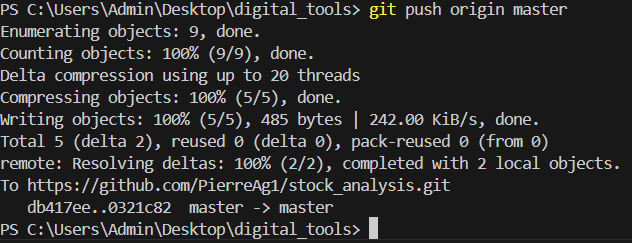
\includegraphics[width=0.9\linewidth]{../images/gitpush.png}
        \caption{Pushing changes on branch master of a Github repository}
        \label{fig:enter-label}
    \end{figure}
\end{frame}


\begin{frame}{Introduction: Repository Structure}
\begin{figure}
    \centering
    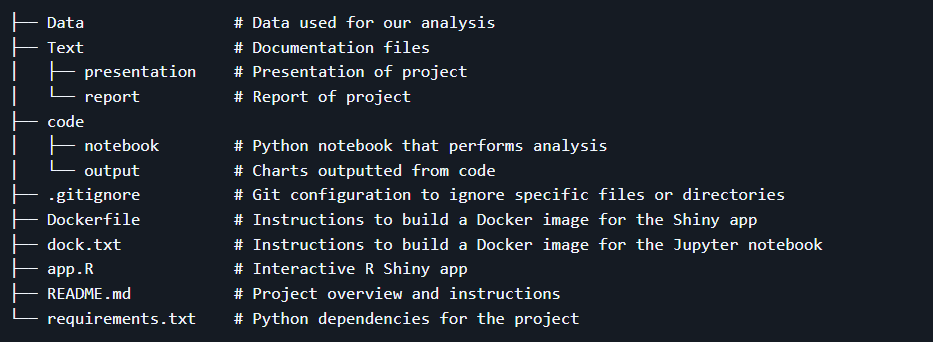
\includegraphics[width=0.9\linewidth]{../images/repo_structure.png}
    \caption{Our Github repository structure}
    \label{fig:enter-label}
\end{figure}
    
\end{frame}


\begin{frame}{Shiny app.R}
\begin{itemize}
    \item Dockerfile
    \item app.R
    \item Results in the browser via Docker Container
\end{itemize}
    
\end{frame}


\section{Data}

\begin{frame}{Data}
  \begin{itemize}
    \item 2 datasets:
      \begin{itemize}
        \item Product announcements dataset retrieved from ChatGPT and official company websites.
        \item Daily stock prices dataset in USD (adjusted for dividends) from 31.12.2013-31.12.2023 for the ten biggest tech firms in terms of current market capitalization compiled with Refinitiv EIKON (Datastream).
      \end{itemize}
    \item Key steps:
      \begin{itemize}
        \item Data Importation, Merging and Cleaning.
        \item Compute Daily Returns \& Rolling Volatility
      \end{itemize}
  \end{itemize}
\end{frame}

\begin{frame}{Data: Libraries Importations}
\begin{itemize}
    \item pandas for data manipulation and analysis
    \item matplotlib for creating visualisations
    \item numpy for numerical computation
    \item seaborn for enhanced statistical visualisations
    \item scikit-learn for statical modeling (linear regression) and for model validation 
\end{itemize}
    
\end{frame}


\begin{frame}{Data: Data Importation, Merging and Cleaning}
  \begin{itemize}
      \item <1->Import both Excel spreadsheets thanks to Pandas library.
      \item <2->Ensure consistency between data types before merging.
      \item <3->Deal with inconsistent or missing values (e.g. zero or negative stock prices).
  \end{itemize}
    
\end{frame}

\begin{frame}{Data: Compute Daily Returns \& Rolling Volatility}
  \begin{itemize}
      \item <1->Computed the daily stock returns and rolling volatility over a 10-day window.
      \item <2->Delete the missing values because the first row of each stock can't provide a daily return and that the 10 day rolling volatility can't be computed before having 10 data points.
      
  \end{itemize}
    
\end{frame}


\begin{frame}{Data: Compute Daily Returns \& Rolling Volatility}
\begin{table}[ht]
    \centering
    \resizebox{\textwidth}{!}{%
        \begin{tabular}{llcccc}
            \toprule
            \textbf{Name} & \textbf{Date} & \textbf{Announcement} & \textbf{StockPrice} & \textbf{Daily\_Return} & \textbf{Rolling\_Volatility} \\
            \midrule
            AMZN & 2014-01-14 & NaN & 20299.90 & 0.016778 & 0.010152 \\
            AMZN & 2014-01-15 & NaN & 20214.63 & -0.004201 & 0.010226 \\
            AMZN & 2014-01-16 & NaN & 20211.05 & -0.000177 & 0.010216 \\
            AMZN & 2014-01-17 & NaN & 20405.61 & 0.009626 & 0.010606 \\
            AMZN & 2014-01-20 & NaN & 20405.61 & 0.000000 & 0.010248 \\
            \bottomrule
        \end{tabular}%
    }
    \caption{Sample of the final dataset}
    \label{tab:final dataset}
\end{table}
\end{frame}

\section{Descriptive Analysis}

\begin{frame}{Descriptive Analysis}
  \begin{itemize}
    \item Descriptive Statistics of the Daily Returns
    \item Cumulative Performance Analysis
    \item Volatility Analysis
    \item Spotting Patterns between Volatility and Product Announcements
  \end{itemize}
\end{frame}


\begin{frame}{Descriptive Analysis: Daily Returns}
  
\begin{table}[ht]
    \centering
    \begin{tabular}{lcccc}
        \toprule
        \textbf{Name} & \textbf{Mean (\%)} & \textbf{Std (\%)} & \textbf{Min (\%)} & \textbf{Max (\%)} \\
        \midrule
        AMZN  & 0.100 & 2.055 & -14.049 & 14.131 \\
        APPL  & 0.109 & 1.758 & -12.865 & 11.981 \\
        AVGO  & 0.151 & 2.156 & -19.913 & 15.834 \\
        GOOG  & 0.077 & 1.727 & -11.634 & 16.259 \\
        META  & 0.098 & 2.315 & -26.390 & 23.283 \\
        MSFT  & 0.112 & 1.675 & -14.739 & 14.217 \\
        NVDA  & 0.230 & 2.872 & -18.756 & 29.807 \\
        TECHY & 0.070 & 2.189 & -12.418 & 23.261 \\
        TSLA  & 0.186 & 3.447 & -21.063 & 19.895 \\
        TSMC  & 0.091 & 1.617 & -8.870  & 10.337 \\
        \bottomrule
    \end{tabular}
    \caption{Descriptive Statistics of the Daily Returns  by firm}
    \label{tab:returns_stats}
\end{table}
    
\end{frame}

\begin{frame}{Descriptive Analysis: Cumulative Performance Analysis}
  
\begin{figure}
    \centering
    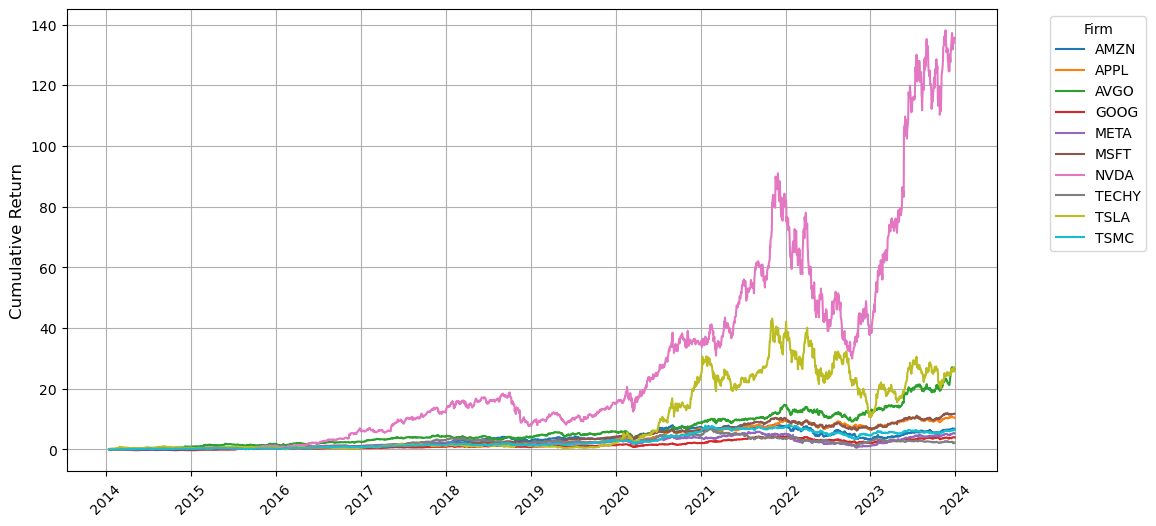
\includegraphics[width=0.9\linewidth]{../images/cum_perf_analysis.png}
    \caption{Cumulative Performance by firm}
    \label{fig:cum_perf}
\end{figure}
    
\end{frame}

\begin{frame}{Descriptive Analysis: Volatility Analysis}
  
\begin{figure}
    \centering
    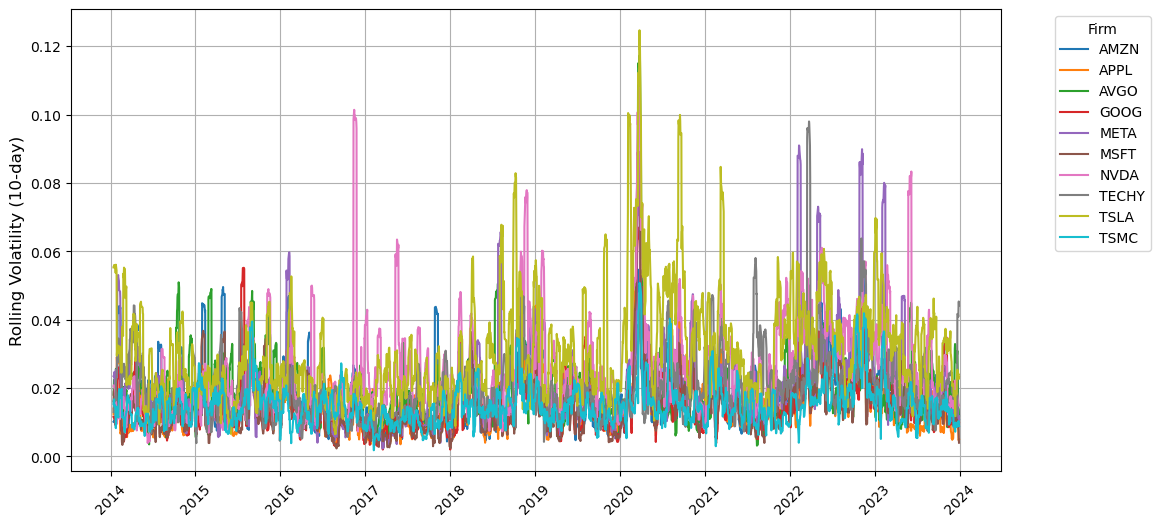
\includegraphics[width=0.9\linewidth]{../images/volatility_analysis.png}
    \caption{Volatility over Time by firm}
    \label{fig:volatility_analysis}
\end{figure}
    
\end{frame}

\begin{frame}{Descriptive Analysis: Spotting Patterns(1)}
  
\begin{figure}
    \centering
    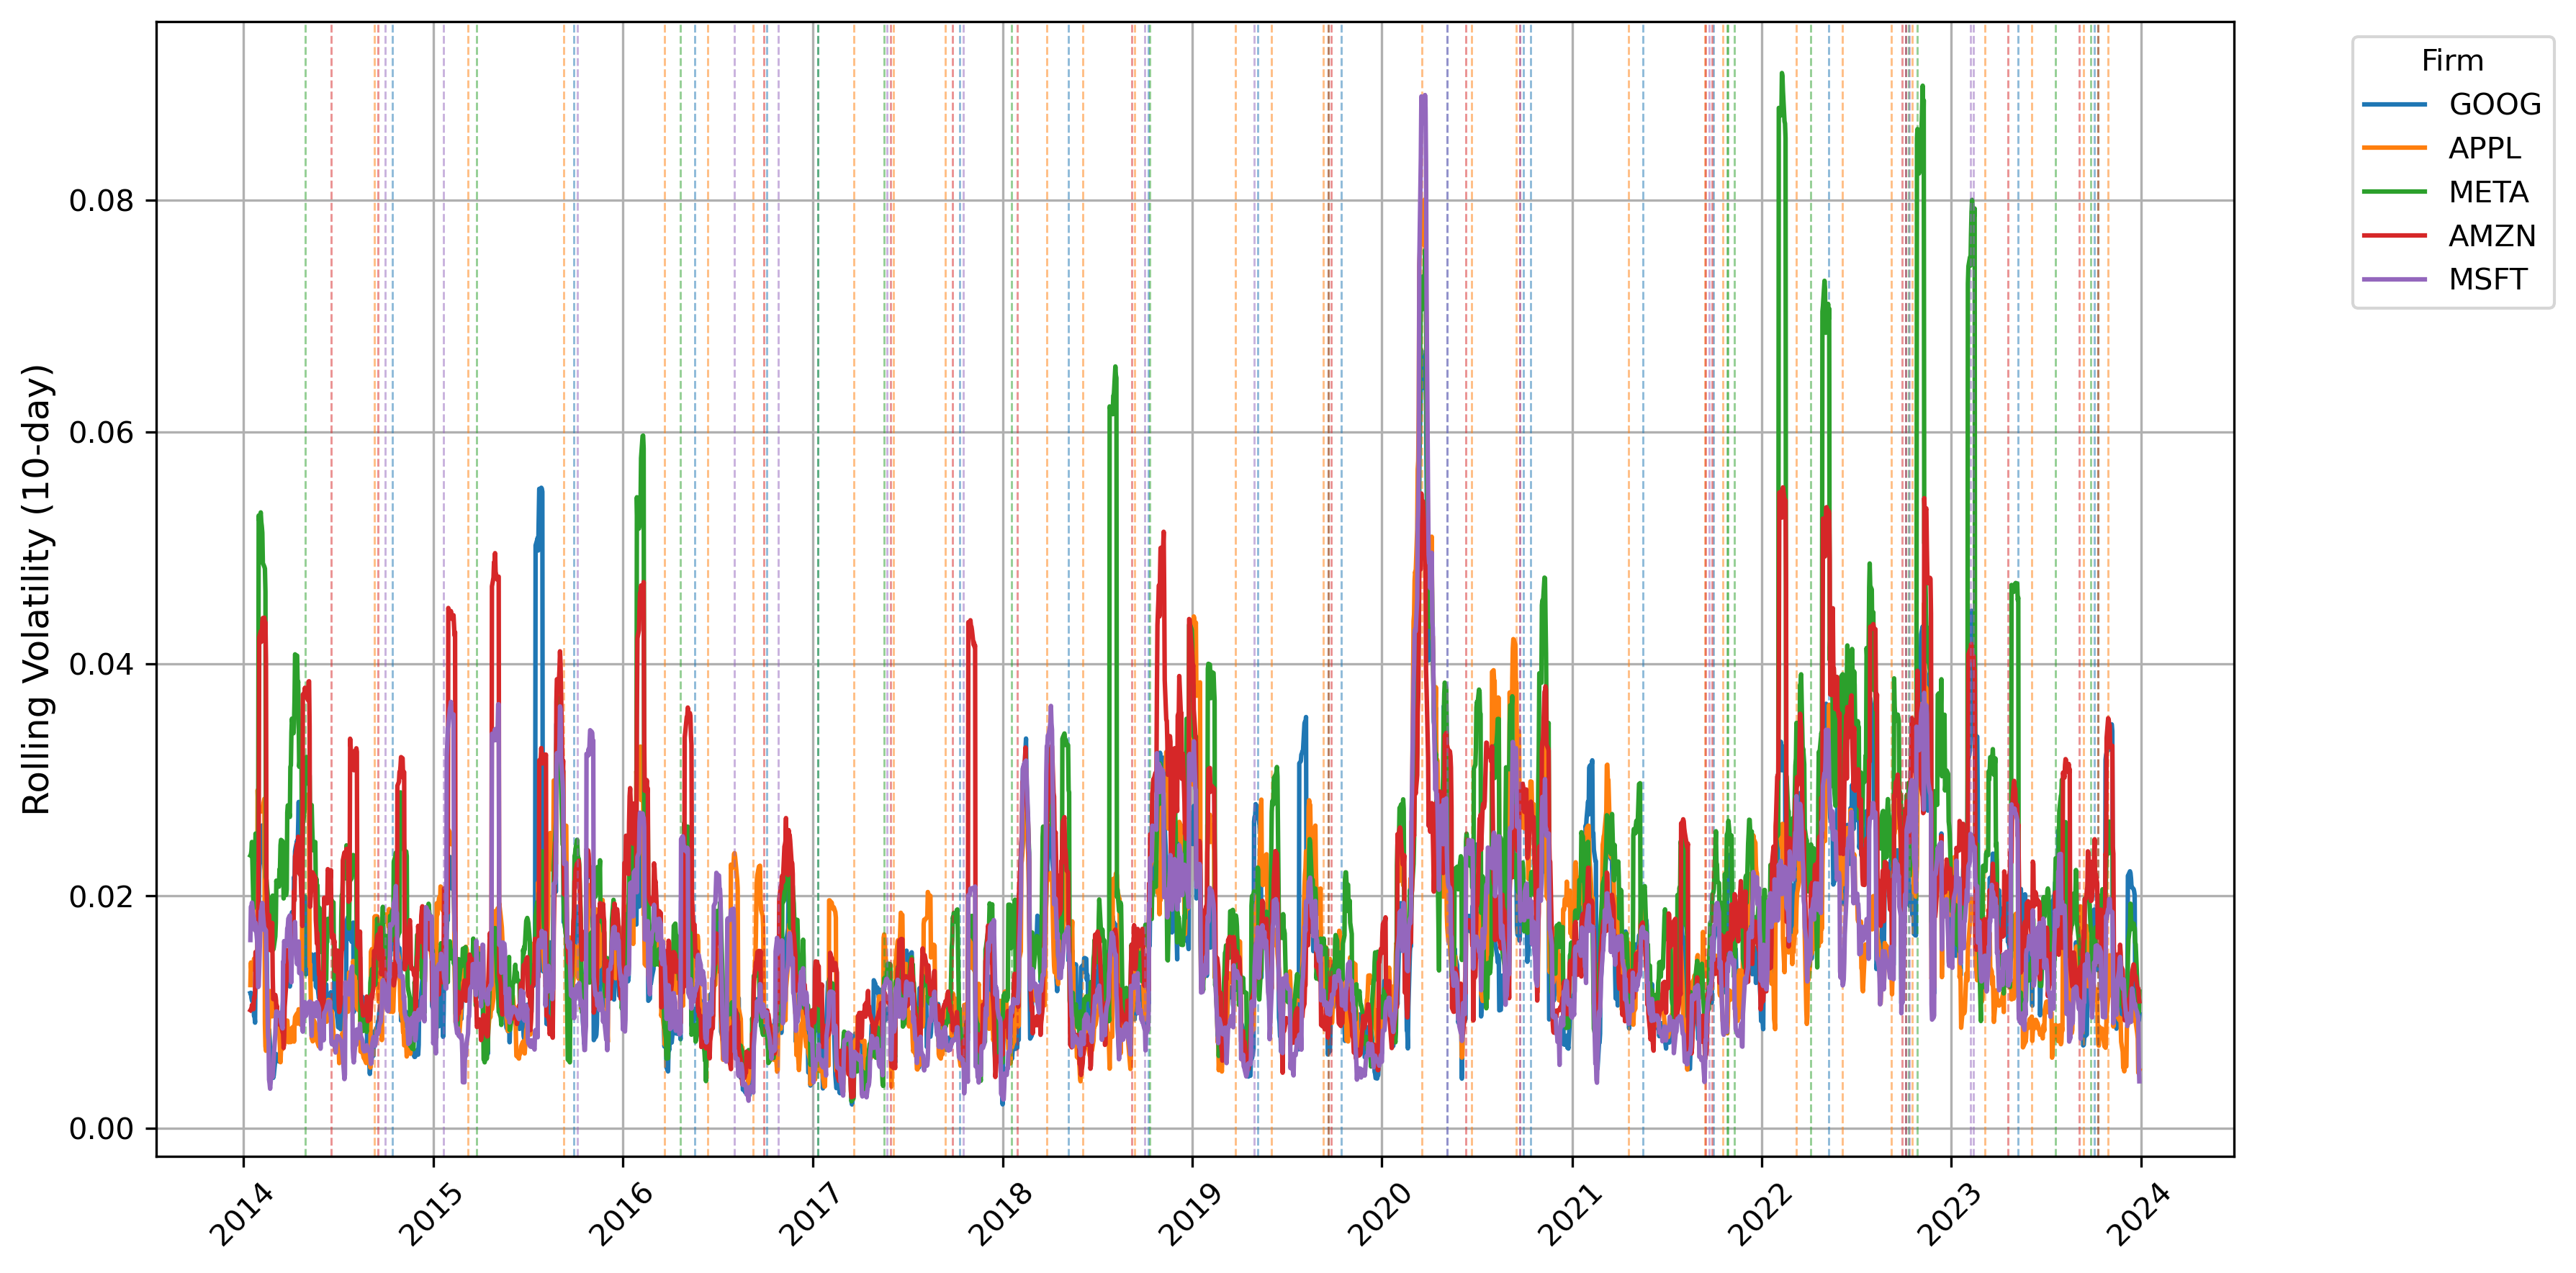
\includegraphics[width=0.9\linewidth]{../images/GAFAM_pattern.png}
    \caption{Volatility and Product Announcements for GAFAM}
    \label{fig:GAFAM_pattern}
\end{figure}
    
\end{frame}

\begin{frame}{Descriptive Analysis: Spotting Patterns(2)}
  
\begin{figure}
    \centering
    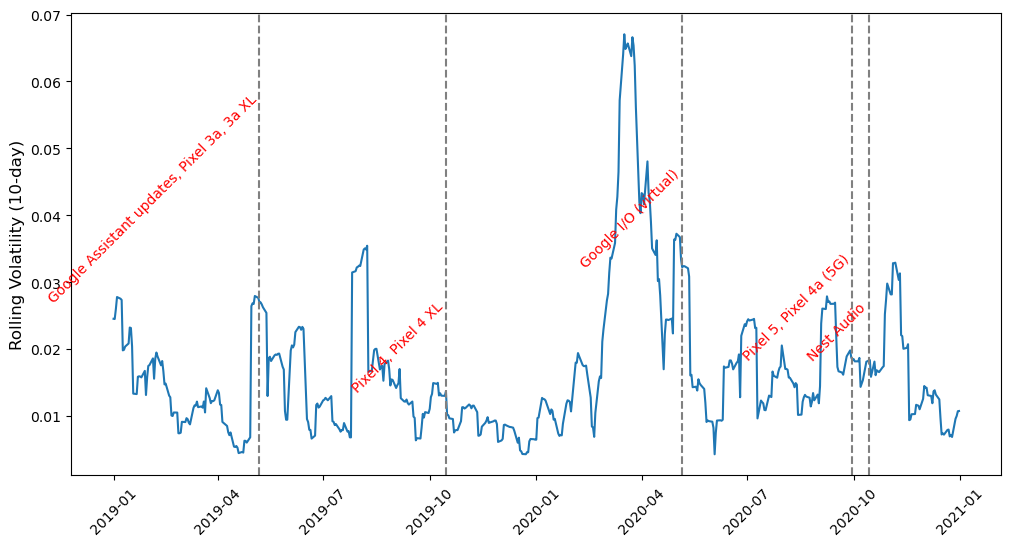
\includegraphics[width=0.8\linewidth]{../images/GOOG_pattern.png}
    \caption{Volatility and Product Announcements during COVID crisis for Google}
    \label{fig:GOOG_pattern}
\end{figure}
    
\end{frame}

\begin{frame}{Descriptive Analysis: Spotting Patterns(3)}
  
\begin{figure}
    \centering
    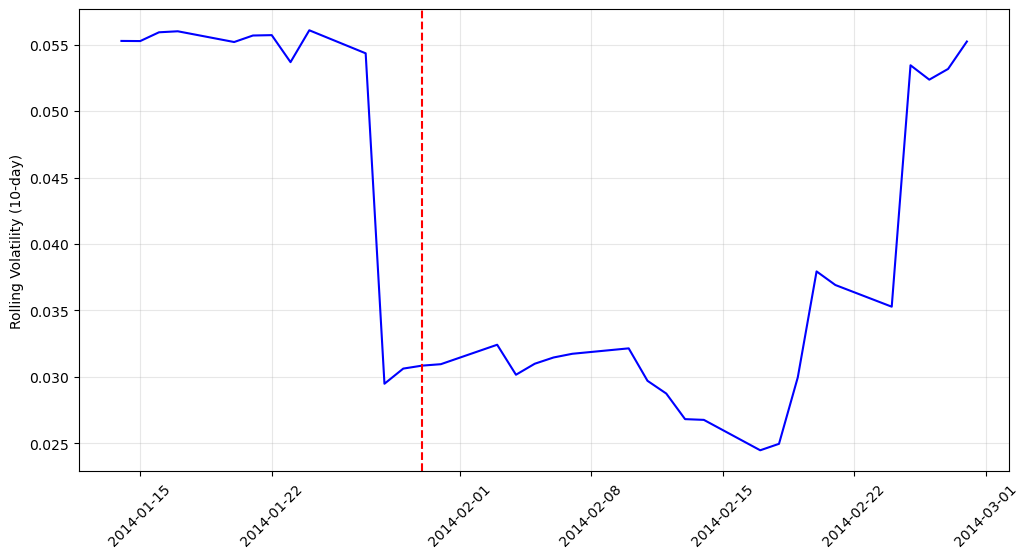
\includegraphics[width=0.8\linewidth]{../images/TESLA_pattern.png}
    \caption{Tesla Stock Volatility around Model S P85D Announcement}
    \label{fig:TESLA_pattern}
\end{figure}
    
\end{frame}


\section{Model}

\begin{frame}{Model}
  \begin{itemize}
    \item Very naive linear model:
    \[
    \text{Rolling\_Volatility}_{it} = \alpha + \beta \cdot \text{Announcement}_{it} + \epsilon_{it}
    \]
    \item Binary independent variable but too few observations.
    \item Absence of control variables to prevent biases.
  \end{itemize}
\end{frame}


\section{Results}

\begin{frame}{Results}

  \begin{table}[ht]
    \centering
    \begin{tabular}{lc}
        \toprule
        \textbf{Parameter} & \textbf{Value} \\
        \midrule
        Intercept & 0.019317437887891822 \\
        Coefficient for Announcement\_Binary & 0.0019166839158981386 \\
        R\(^2\) Score & -0.0005099587924510818 \\
        \bottomrule
    \end{tabular}
    \caption{Regression Results}
    \label{tab:regression_outputs}
\end{table}

\end{frame}


\section{Conclusion}

\begin{frame}{Conclusion}
  \begin{itemize}
    \item Limitations \& Future Improvements
    \item Business Implications
  \end{itemize}
\end{frame}

\begin{frame}{Conclusion: Limitations \& Future Improvements}
  \begin{itemize}
    \item Hard to know where the impact exactly takes place: for example, is it when the product is announced or released?
    \item Finding control variables is not easy but factors such as changes in interest rates, geopolitical events, and general economic conditions could have a significant impact on volatility and affect product announcements of firms.
    \item Asymmetry between stock returns computed daily and products announced only several times in a year.
    \item Is rolling volatility a good measure in our case? Window size?
    \item Trade-off between interesting subjects and data accessibility.
  \end{itemize}
\end{frame}

\begin{frame}{Conclusion: Business Implications}
  \begin{itemize}
    \item  Investors need to consider a broader range of factors beyond announcements when evaluating stock price movements.
    \item Companies can focus on product strategy and innovation without excessive concern for short-term market reactions.
    \item Our findings challenge the logical assumption that major product announcements significantly affect stock behavior, emphasizing the importance of a more comprehensive approach when analyzing market dynamics.
  \end{itemize}
\end{frame}



\end{document}
